% -*- mode: LaTeX; coding: utf-8; -*-

\chapter{Perinteiset tietoturvahyökkäykset}

Tietoyhteiskunnassa yksikään verkossa oleva laite ei ole suojassa
tietoturvahyökkäyksiltä, ja niiden mukanaan tuomilta
ongelmilta. Hyökkäykset ovat nykyisin myös hyvin monimuotoisia ja ne
voidaan jakaa eri kategorioihin niiden tavoitteiden ja toteutustapojen
mukaan. Uusia hyökkäystapoja kehitetään jatkuvasti lisää ja
tunnetutkin hyökkäystavat saavat uusia ominaisuuksia. Vaikka
suurimpaan osaan hyökkäyksistä on olemassa erilaisia
suojautumistapoja, on näiltä kaikilta suojautuminen ylläpitäjän
kannalta mahdoton tehtävä. Verkon turvallisuuden kannalta on kuitenkin
tärkeää, että hyökkäysten riskit tiedostetaan ja uhkien toteutumisen
todennäköisyyksiä voidaan pienentää mahdollisuuksien ja resurssien
rajoissa.


\section{Tiedon urkinta ja väärentäminen}

Ennen kuin hyökkääjä pystyy murtautumaan verkkoon tai verkossa
sijaitsevaan tietokoneeseen, tulee hänen selvittää järjestelmän
mahdolliset heikkoudet. Haluttuja tietoja ovat esimerkiksi asennetut
käyttöjärjestelmät, ohjelmistojen versiotiedot sekä verkon yleinen
rakenne ja tietoturvataso. Näiden tietojen selvittämiseksi hyökkääjä
aloittaa verkkoa kohtaan joukon hyökkäyksiä, joita kutsutaan
tiedusteluhyökkäyksiksi (engl. \textit{Probe Attacks}). Tällaiset
tiedustelut ovat varsinaisia hyökkäyksiä yleisempiä, sillä niiden
toteuttaminen ei vaadi hyökkääjältä kovin syvällistä
osaamista. Verkosta löytyy paljon valmiita työkaluja, joiden avulla
hyökkääjä pystyy urkkimaan tarvittavat tiedot ja mahdollisesti jo
saman tien hyödyntämään havaittuja heikkouksia. Hyökkääjä, jolla on
tietämystä verkossa käytettävistä laitteista ja palveluista, voi
hyödyntää näitä tietoja haavoittuvuuksien etsimiseen ja järjestelmien
murtautumiseen \cite{IDS}.

Kun hyökkääjällä on riittävä tietämys verkon eri komponenteista, voi
hän aloittaa hyökkäyksen suunnittelun. Yksi tapa murtautua
tietoverkkoon on hyödyntää verkkokerroksen protokollissa, kuten TCP ja
IP, olevia heikkouksia. Tällaisia hyökkäyksiä kutsutaan
\textit{spoofing}- eli \textit{petkutushyökkäyksiksi}. Niissä
murtautuja pyrkii naamioimaan oman koneensa siten, että se näyttäa
kuuluvan kohteena olevan laitteen kanssa samaan lähiverkkoon.  Tällöin
hyökkääjä pystyy helpommin huijaamaan kohdekonetta jakamaan ja
lähettämään arkaluontoista tietoa, jota jaettaisiin muuten ainoastaan
luotettujen osapuolien kesken.  Tällaiset hyökkäykset jaotellaan
edelleen sokeisiin ja aktiivisiin hyökkäyksiin sen mukaan, kuinka
paljon hyökkääjällä on tietoa verkon rakenteesta. Sokeassa
hyökkäyksessä kohdekoneen lähettämiä vastauksia ei pystytä seuraamaan,
koska murtautujan oikeudet ovat puutteellisia ja IP-osoite, jonka
haltijaksi hyökkääjä haluaa naamioitua, on harvoin tiedossa.
Aktiivisessa hyökkäyksessä murtautujalla on käytettävissään tietoa
tietokoneiden välisistä käyttöoikeuksista, jolloin tiedon
korruptoiminen, muokkaaminen ja välittäminen toiseen verkkoon on
helpompaa toteuttaa \cite{WEBS}.

\subsection{IP Spoofing}

IP Spoofing on hyökkäys, jossa pyritään murtautumaan verkkoon ja
hankkimaan arkaluontoista tietoa väärentämällä lähetettäviin
paketteihin luotetun koneen IP-osoite. Hyökkäykset jaotellaan
sokeisiin ja aktiivisiin hyökkäyksiin sen mukaan, mistä hyökkäys
toteutetaan. Hyökkäykset toimivat siten, että kolmivaiheisen
yhteydenmuodostuksen aikana hyökkääjä tekeytyy tietokoneeksi, johon
hyökkäyksen kohteella on luottamussuhde. Tämä tapahtuu muokkaamalla
lähetettävien pakettien otsaketietoja ja kuittausnumeroita. Tässä
onnistuakseen hyökkääjän tulee pystyä vastaamaan oikeilla
kuittausnumeroilla kohteen lähettämiin paketteihin. Nämä
kuittausnumerot hyökkääjä joutuu aluksi usein arvaamaan, jonka vuoksi
tämä hyökkäystapa on vaikea toteuttaa \cite{WEBS}. Niin kutsuttu Man
in The Middle -hyökkäys, jossa hyökkääjä kaappaa kahden koneen välisen
yhteyden, perustuu myös IP-\-osoitteen väärinkäyttöön. Kuva \ref{Man}
havainnollistaa hyökkäyksen toteuttamista.

\begin{figure}[ht]
\centering
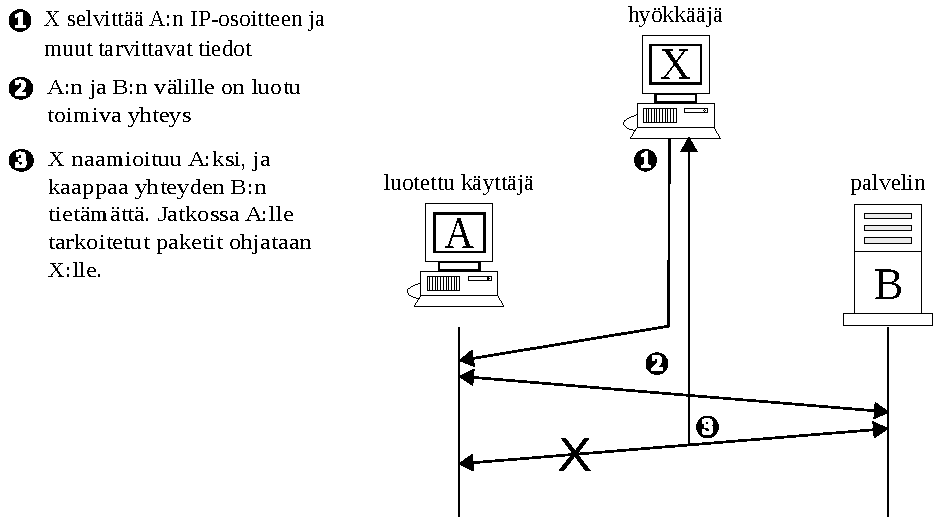
\includegraphics[width=13cm]{pics/MiTM.pdf}
\caption{Man in The Middle-hyökkäys}
\label{Man}
\end{figure}

Vaikka IP-osoitteen väärentämiseen perustuvat hyökkäykset ovat
vaikeita toteuttaa, ovat ne melko yleisiä, sillä jokainen
TCP/IP-protokollaa käyttävä järjestelmä on niille alttiina. Tämä
johtuu siitä, että TCP/IP-verkossa on sallittua muokata paketteja
tiedonsiirron aikana. Näin on, koska eräät IP-pohjaiset palvelut
edellyttävät pakettien sisällön muuttamista lähettämisen
yhteydessä. Tällaisia palveluita ovat esimerkiksi mobiili-IP- ja
VPN-järjestelmät.~\cite{DDOS}.

IP spoofing -hyökkäyksiä voidaan torjua monin eri keinoin. Tehokkain
tapa on määritellä verkon reitittimet estämään sellaisten pakettien
kulku, jotka on merkitty lähetetyiksi sisäverkon laittelta, mutta
jotka todellisuudessa saapuvat reitittimeen sen ulkopuolisista
liitännöistä. Jos tämä kuitenkin halutaan sallia, niin jokainen sessio
tulisi kryptata reitittimessä. Muutenkin yhteyksien muodostumisen
tulisi pohjautua koko järjestelmän kattavaan salaukseen \cite{WEBS}.

% TODO: tarkista, mitä tällä kryptaamisella reitittimessä oikein
% tarkoitetaan. Tarkistetaan lähteestä.

\subsection{ARP Spoofing}

Nykyisin lähes jokainen verkko pohjautuu TCP/IP-protokollan ja
Ethernet-verkon väliseen yhteistoimintaan. Tässä yhteydessä tarvitaan
ARP-pro\-to\-kol\-laa, jonka tehtävänä on selvittää IP-osoitteita
vastaavat Ethernet- eli MAC-osoiteet. Ethernet-osoite
verkkokorttikohtainen ja sen avulla yksilöidään lähiverkossa
sijaitsevat tietokoneet ja muut aktiivilaitteet.  Tietoa tarvitaan
myös IP-protokollalla liikennöitäessä, koska ilman tietoa
Ethernet-osoitteesta lähiverkossa sijaitseva reititin ei pystyisi
välittämään Internetistä saapuvia paketteja eteenpäin oikealle
laitteelle eikä myöskään lähiverkossa sijaitseva tietokone pystyisi
siirtämään tietoa IP-protokollalla muille lähiverkossa sijaitseville
laitteille.

ARP spoofing -hyökkäyksessä, jota kutsutaan myös ARP-myrkyttämiseksi,
pyritään syöttämään syöttämään reitittimien ARP-tauluihin virheellistä
tietoa (kuva \ref{ARP-spoofing}). Tämä tapahtuu kaappaamalla verkon
yleislähetysviestejä ja muokkaamalla kuittausviestien sisältöä siten,
että kuittausviesteihin hyökkääjä laittaa kohdeosoitteeksi oman
IP-osoitteensa. Verkon aktiivilaitteilta saapuviin, muille
tarkoitettuihin kyselyihin vastataan omalla MAC-osoitteella.  Tämän
jälkeen kohdelaitteelle tarkoitetut paketit ohjautuvatkin hyökkääjän
koneelle \cite{WEBS}.

ARP-protokolla on hyvin haavoittuvainen hyökkäyksille, koska
oletuksena se ei sisällä minkäänlaista suojautumiskeinoa
ARP-myrkyttämiselle. Siksi paras keino suojautua tällaisilta
hyökkäyksiltä on varmistaa, että ennen ARP-taulun muokkausta
tunnistetaan käyttäjät jollakin keinolla. Toinen mahdollisuus on
käyttää verkkolaitteissa staattisia ARP-tauluja~\cite{WEBS}. Jakamalla
lähiverkko pienempiin osiin virtuaalisten lähiverkkojen (VLAN) avulla
voidaan myöskin rajata ARP-myrkyttämisen vaikutuksia.

\begin{figure}[ht]
\centering
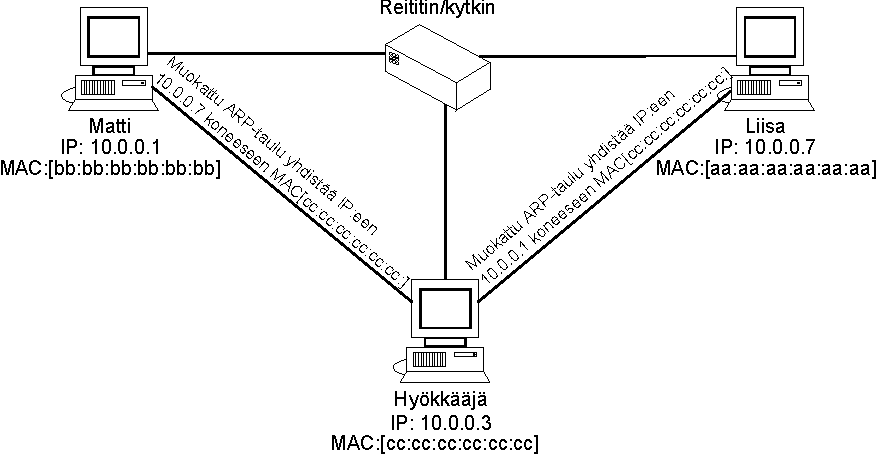
\includegraphics[width=12cm]{pics/arp.pdf}
\caption{ARP-taulun myrkyttäminen käyttäen Man In the Middle -hyökkäystä.}
\label{ARP-spoofing}
\end{figure}

\section{Denial Of Service}

CERT \cite{CERT}, joka on yksi tietoturva-alan johtavista
tutkimuskeskuksista, määrittelee palvelunestohyökkäyksen
(engl. \textit{Denial of Service}, DoS) sellaiseksi teoksi, jossa
hyökkääjän tavoitteena on estää palvelun käyttäjiä käyttämästä heille
kuuluvia tai heidän käytettävissään olevia palveluita. Tällaisia
palveluita voivat olla esimerkiksi tietoliikenneresurssit tai verkossa
käytettävät Web-sovellukset. Hyökkäyksillä pyritään lamauttamaan
palvelua tarjoava verkko tai palvelin siten, että asiaankuuluvien
pyyntöjen vastaanottamiseen tai käsittelyyn ei enää riitä
resursseja. Keinoja hyökkäysten toteuttamiseen on monia. Koska
valtaosa palvelunestohyökkäyksistä käyttää hyväkseen eri protokollien
sallittuja toimintoja, on hyökkäyksiltä suojautuminen hyvin vaikeaa
\cite{Hacking}.

Palvelunestohyökkäykset voidaan jakaa kolmeen ryhmään näiden
toteutustapojen ja tavoitteiden mukaan. Ensimmäiseen ryhmään kuuluvat
hyökkäykset, joiden tarkoituksena on kuormittaa palvelimia ja kuluttaa
loppuun niiden rajoitetut resurssit. Tämä voidaan toteuttaa esimerkiksi
kuormittamalla verkkoa tai palvelinta turhilla pyynnöillä. Toiseen
ryhmään kuuluvat hyökkäykset, jotka pyrkivät joko tuhoamaan tai
muuttamaan konfigurointitietoja siten, että kone tai verkko lakkaa
toimimasta. Viimeiseen ryhmään kuuluvat verkon komponenttien
muokkaamiseen tai tuhoamiseen tähtäävät hyökkäykset
\cite{CERT}. Vaikka tässä työssä keskitytään vain resursseihin
kohdistuviin hyökkäyksiin, niin palvelun kokonaisturvallisuuden
kannalta ylläpitäjän tulee kiinnittää jokaiseen ryhmään tasapuolisesti
huomiota.

Viime vuosina palvelunestohyökkäysten kirjo on voimakkaasti
laajentunut. Alkuperäisten, pelkästään verkkokerroksen raa’an voiman
hyökkäysten, lisäksi on alkanut esiintyä sovelluskerroksen
hyökkäyksiä, joiden toteuttaminen vaatii hyökkääjältä usein varsin
vähän omia resursseja \cite{Hacking}. Nämä sovelluskerroksen
hyökkäykset ovat toteutukseltaan hyvin hienostuneita, jolloin ne
jäävät yleensä huomaamatta tavanomaisilta tietoturvajärjestelmiltä,
koska tietoliikenteen sisältö ei juurikaan poikkea
normaalitilanteesta. Hyökkääjä saattaa esimerkiksi pyytää sellaista
resurssia palvelulta, jonka kysely vie vain vähän hyökkääjän omia
resursseja, mutta aiheuttaa palvelimelle suuren kuormituksen
\cite{DDOSb}.

Sovelluskerroksen hyökkäysten teho nähtiin vuonna 2004, kun
MyDoom-\-viruksella saastuneet koneet kuormittivat yleisimpiä
hakukoneita etsimällä näiden avulla uusia sähköpostiosoitteita, joihin
lähettää saastunut sähköposti \cite{Hacking}. Sovelluskerroksen
hyökkäyksen vaikutus voidaan kohdistaa myös yksittäisiä palveluita
kohti, jolloin vaikutukset ovat vieläkin suuremmat. Näin tapahtui
vuonna 2003, kun Yhdysvalloissa yrittäjä palkkasi ns. DDoS-mafian
kaatamaan kilpailijoidensa verkkosivut HTTP-kyselyillä, jotka pyysivät
ladattavaksi isoa kuvatiedostoa \cite{DDOSb}. Tämä aiheutti kolmelle
kilpailijalle arviolta jopa miljoonan dollarin tappiot ja pysäytti
näiden liiketoiminnan lähes kahdeksi viikoksi \cite{FBI}.

\subsection{SYN-hukuttaminen}
TCP/IP-protokollan yksi suunnittelulähtökodista oli, että sitä
käytettäisiin avoimessa ja luotetussa ympäristössä. Tästä syystä sen
suunnittelussa ei osattu ottaa huomioon mahdollisia vihamielisiä
käyttäjiä, jotka pyrkisivät häiritsemään muiden käyttäjien
tietoliikennettä. TCP/IP-protokollan käyttö julkisissa verkoissa kuitenkin
yleistyi arvaamattomasti, jonka vuoksi suunnitteluvaiheessa tehdyt
virheet periytyivät nyt käytössä olevaan IPv4-verkkojen rakenteisiin
\cite{Hacking}.

Yhteydenmuodostus TCP-protokolla tapahtuu kolmivaiheisesti. Aluksi
yhdistävä tietokone lähettää palvelimelle SYN-paketin, jonka
seurauksana palvelin varaa tulevalle yhteydelle resursseja ja lähettää
yhdistävälle tietokoneelle SYN/ACK-paketin. Tämän jälkeen palvelin
jää odottamaan yhteyden muodostamista. Tähän yhdistävän tietokoneen
tulee vastata ACK-paketilla, jonka jälkeen yhteys on muodostunut ja
tiedonsiirto voi alkaa \cite{Hacking}. Tunnetuin TCP:tä käyttävä
protokolla on Webissä käytettävä HTTP. Sen avulla Web-palvelimet
pystyvät nopeasti palvelemaan useita yhtäaikaisia käyttäjiä.

TCP/IP-protokollan historiasta perityistä heikkouksista tunnetuin ja
käytetyin on SYN-hukuttamiseksi kutsuttu hyökkäys, jossa hyökkääjä
pyrkii kuluttamaan kohteen tietoliikennekapasiteetin loppuun
tekaistuilla yhteydenmuodostuspyynnöillä. Hyökkäys on hyvin
yksinkertainen ja helppo toteuttaa, sillä se käyttää hyväkseen
TCP-protokollaan määritettyjä toimintoja. Hyökkäyksessä
TCP-protokollan kolmiosaista yhteydenmuodostusta ei viedä loppuun
saakka vaan jätetään palvelin odottamaan ACK-paketti yhdistävältä
tietokoneelta.

Koska TCP-protokolla pyrkii aina varmistamaan yhteyden muodostumisen,
lähetetään SYN/ACK-paketti tarvittaessa uudestaan, kunnes yhdistävä
tietokone vastaa ACK-paketilla tai määritelty aikaraja tulee
vastaan. Tätä ominaisuutta hyökkääjä pystyy käyttämään
hyväkseen. Riittää, että hyökkääjä nuuskii selville käyttämättömän
IP-osoitteen, joka on vielä mieluiten samasta aliverkosta kuin missä
palvelin sijaitsee. Tämän jälkeen hyökkääjä luo SYN-paketin, jossa on
tämä tekaistu IP-osoite. Koska palvelimen lähettämä SYN/ACK-viesti ei
koskaan saavu oikealla koneelle, ei palvelin saa ACK-kuittausta. Tällöin
TCP-protokolla alkaa lähettämään pakettia uudestaan niin kauan
kunnes määritetty raja yhteyden aikakatkaisulle tulee vastaan
\cite{STACK}. Hyökkääjän on vaivatonta automatisoida nämä vaiheet ja
hyökkäys voidaan toteuttaa esimerkiksi saastuneista koneista
muodostetun verkoston avulla. Näin saadaan aikaiseksi kuvan \ref{syn}
mukainen tilanne, jossa useita IP-osoitteita käyttämällä hyökkääjä
häiritsee kohteen toimintaa turhilla yhteydenottopyynnöillä.

\begin{figure}[hpt]
\centering
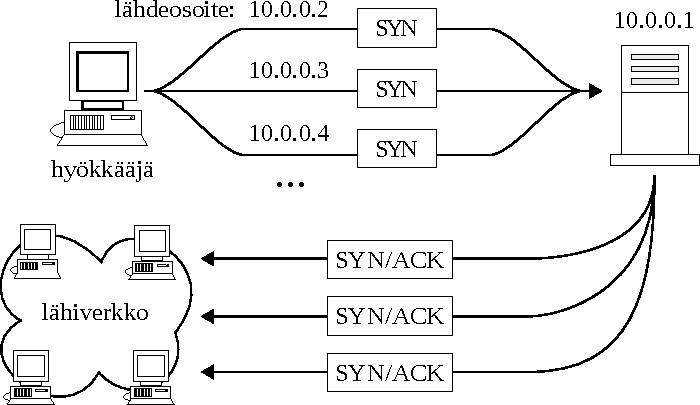
\includegraphics[width=12cm]{pics/syn.pdf}
\caption{SYN-hyökkäys käyttäen useita lähiverkon IP-osoitteita.}
\label{syn}
\end{figure}

SYN-hukuttamisen mahdollistavan mekanismin avulla voidaan myös toteuttaa
heijastettu hyökkäys (engl. \textit{reflective attack}), joka on muunnos 
SYN-hukuttamisesta. Tässä hyökkäyksessä väärennetyissä SYN-viesteissä on
lähettäjäksi merkitty haluttu kohde. Lähettämällä suuri määrä näitä SYN-viestejä 
esimerkiksi Web-\-palvelimelle, aiheutuu vastaustulvasta ongelmia
kohteelle \cite{STACK}.

Koska ylimääräistä palvelinkapasiteettia ei useinkaan ole järkevää
pitää SYN-\-hukuttamisen varalta, joudutaan ratkaisua
hakemaan muualta. Alkeellisin keino on rajoittaa puoliavonaisten
yhteyksien määrää, jolloin rajan ylittyessä yhteyksiä aletaan
pudottamaan \cite{TCP}. Toinen käytetty keino on reitittimiltä
verkkoon päin tulevan liikennemäärän seuraaminen ja liikennepiikkeihin
reagoiminen. Hyökkäyksiä vastaan voidaan myös suojautua liikenteen
seuraamiseen tarkoitetuilla sovelluksilla sekä pääsylistoilla
\cite{STACK}.

Kehittyneempi suojautumiskeino on muuttaa TCP-protokollan kättelyä
siten, että yhteyden tarvitsemat resurssit varataan vasta ACK-viestin
vastaanottamisen yhteydessä. Tätä menetelmää kutsutaan
SYN-evästykseksi (engl. \textit{SYN Cookies}) ja se on tuettu
mm. Linuxissa ja FreeBSD:ssä~\cite{syncookies}. Yhteydenmuodostuksessa
tarvittavat parametrit kätketään tällöin SYN-paketin
järjestysnumeroon. Tämän menetelmän käyttö kuitenkin rajaa pois
runsaasti TCP-protokollan ominaisuuksista, jonka vuoksi SYN-evästys
kytketään yleensä päälle vain hyökkäysten ajaksi.

Täydellistä ratkaisua SYN-hukuttamista vastaan ei mikään näistä
tavoista kuitenkaan tarjoa. Huolellisesti toteutettua hyökkäystä on
vaikea torjua.

\subsection{UDP Echo}

Myös UDP-protokollan käyttö mahdollistaa hyökkäysten tekemisen. Nämä
hyökkäykset käyttävät hyväkseen UDP Echo -protokollaa, mikäli sen
käyttö on sallittu verkossa. Näistä hyökkäyksistä tunnetuin on
Fraggleksi nimetty hyökkäys, joka nykyisinkin aiheuttaa väärin
konfiguroidussa verkossa suuria ongelmia.  Fraggle toimii siten, että
hyökkääjä lähettää UDP Echo -viestin yleislähetyksenä, johon on
merkitty lähettäjäksi hyökkäyksen kohde. Tähän viestiin kaikki verkon
koneet pyrkivät vastaamaan, jolloin kohdetietokoneen
tietoliikennekapasiteetti ja resurssit käytetään viestien
vastaanottamiseen (kuva \ref{fraggle}).

Fraggle on hyvä esimerkki vahvistetusta hyökkäyksestä, jossa verkon
laitteiden määrä vaikuttaa siihen, kuinka vakava hyökkäys on
\cite{WEBS}. Vastaavanlainen hyökkäys voidaan myös toteuttaa kahden
koneen välillä, jos kummassakin on sallittuna UDP Echo
-viestit. Tällöin hyökkääjä väärentää viestiin lähettäjän osoitteen ja
halutun kohdeportin. Vastaanottaja vastaa tähän viestiin omalla
Echo-viestillä, ja näin kahden koneen välille muodostuu ikuinen
silmukka \cite{TCP}.

\begin{figure}[htp]
\centering
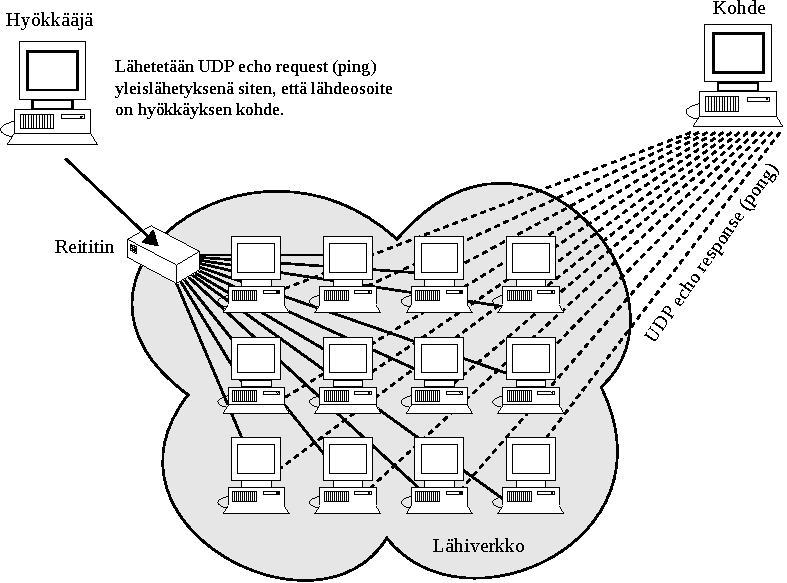
\includegraphics[width=13cm]{pics/fraggle.pdf}
\caption{Vahvistettu UDP Echo -hyökkäys.}
\label{fraggle}
\end{figure}

\subsection{Smurf}

Smurf on yksi ensimmäisistä vahvistetuista DoS-hyökkäyksistä, ja se
toimii lähes identtisesti Fragglen kanssa sillä erolla, että UDP:n
sijasta käytetään ICMP-\-protokollaa. Hyökkääjä lähettää kohteen
puolesta yleislähetyksenä verkolle ICMP Echo -paketin, johon verkon
laitteet vastaavat, jos Echo-viestit on sallittuja verkossa. Jo 100
tietokoneen lähiverkko pystyy aiheuttamaan 14 Mb/s haittaliikenteen
kohdekoneelle, joten pienessäkin väärin konfiguroidussa verkossa
on mahdollista muodostaa riittävästi haittaliikennettä tietoliikenteen
häiritsemiseen tai estämiseen \cite{Hacking}.

Jos hyökkäys on päässyt käyntiin, ei tälle ole paljoa muuta tehtävissä
kuin poistaa kohteena olevat laitteet pois verkosta. Paras vastatoimi
Fragglen ja Smurffin kaltaisille hyökkäyksille on konfiguroida verkon
laitteet alusta asti oikein. ICMP Echo -yleislähetysten estämisellä
pääsee jo pitkälle. ICMP-protokollan käyttöä verkossa kannattaa
muutenkin tarkkailla ja tarvittaessa rajoittaa \cite{Hacking}.

\section{Distributed Denial of Service}

Vielä viime vuosikymmenellä palvelunestohyökkäykset perustuivat
yleensä käyttöjärjestelmistä löydettyjen heikkouksien
hyödyntämiseen. Näiden hyökkäysten aikaansaama tuho riippui paljon
käytettävistä järjestelmistä ja vahingot olivat melko
rajattua. Palvelunestohyökkäyksiä ei nähty tällöin kovinkaan vakavana
uhkana, mutta suhtautuminen muuttui 2000-luvulle tultaessa, kun
hajautetut palvelunestohyökkäykset (engl. \textit{Distributed Denial
of Service}) kehitettiin. Tällaisessa hyökkäyksessä palvelua saattaa
olla lamauttamassa jopa yli 140~000 saastunutta konetta. Tällaisia
saastuneita koneita kutsutaan zombeiksi (engl. \textit{zombie}).

Tietokone voidaan muuttaa zombiksi murtautumalla ja asentamalla siihen
ohjelmisto, jonka avulla murtautuja pystyy hallitsemaan laitetta
käyttäjän tietämättä. Zombiverkoston ei tarvitse edes olla kovinkaan
suuri aiheuttaakseen tuhoa, sillä jo 3~000 koneen verkosto, jossa
jokainen kone tuottaa 25 kb/s liikennettä, aiheuttaa yhteensä 75 Mb/s
kuormituksen verkolle \cite{Hacking}.  Palvelunestohyökkäyksen
seuraamukset ovat varautumattomalle taholle usein katastrofaaliset ja
pahimmillaan hyökkäys saattaa pysäyttää organisaation toiminnan
useiksi päiviksi \cite{CERT}.

Hyökkäysten hajauttaminen useammalla koneelle tuo useita hyötyjä
verrattuna perinteiseen palvelunestohyökkäykseen, jossa hyökkäys
toteutetaan käyttäen yhtä konetta. Otetaan esimerkiksi vaikka
Web-palveluita tarjoava palvelin, jota vastaan halutaan tehdä
palvelunestohyökkäys. Tällaisella palvelimella on käytössä
huomattavasti suurempi määrä resursseja (tietoliikennekapasiteetti,
muisti, laskentateho) kuin yksittäisellä zombitietokoneella on. Kun
hyökkäys suoritetaan yhtäaikaisesti useammalla koneella, pystyy
hyökkääjä kuluttamaan suuretkin resurssit loppuun lyhyessä
ajassa. Yksittäiseltä koneelta tuleva palvelunestohyökkäys on helppo
tunnistaa ja estää verkon ylläpitäjän toimesta. Hyökkääjien määrän
kasvaessa tehtävä vaikeutuu huomattavasti, koska haittaliikennettä
aiheuttavat tietokoneet tai itse haittaliikenne pitää tunnistaa
hyötyliikenteen joukosta. Mikäli zombitietokoneet ovat sijoittuneet ympäri
Internetiä, on hyökkäysten pysäyttäminen ilman palvelun laadun heikkenemistä
mahdoton tehtävä ilman automatisointia. Haittaliikennettä on tällöin myös
vaikea erottaa tavallisesta liikenteestä, koska se tulee palvelimelle
useita reittejä pitkin \cite{DDOS}.

Nopeiden yhteyksien ja verkossa olevien tietokoneiden räjähdysmäinen
kasvu on tehnyt hajautetuista palvelunestohyökkäyksistä hyvin
tehokkaita ja tuhoisia. Suuri määrä verkkoon liitetyistä laitteista on
huonosti suojattu ja päivitetty, ja ihmisten tietoisuus verkon
vaaroista on usein puutteellista. Tämä on luonut otollisen maaperän
suurten zombiverkostojen muodostamiselle virusten ja matojen
avustuksella. Tarjolla on myös tätä tarkoitusta varten suunniteltuja
työkaluja ja ohjelmistoja, jotka tekevät tarvittavat toimenpiteet
automaattisesti. Jo ensimmäiset, vapaasti saatavilla olevat työkalut,
kuten Trinoo ja Shaft, mahdollistivat tuhansien suojaamattomien
koneiden haltuunoton ilman suurempaa perehtymistä \cite{DDOS}.

Hyökkäyksessä käytetyt koneet voidaan jakaa agentteihin (engl. \textit{agents})
ja liikenteen ohjaajiin (engl. \textit{handlers}) riippuen näiden
rooleista. Näistä koneista hyökkääjä käskyttää suoraan liikenteen
ohjaajia, jotka ohjaavat edelleen annetut käskyt agenteille
hyökkäyksen alettua \cite{WEBS}\cite{DDOS}. Ensimmäisissä 
DDoS-verkoissa nämä ohjausviestit olivat salaamattomia, jolloin kuka tahansa
pystyi kaappaamaan näitä. Tämä oli tietomurtojen tekijöiden
näkökulmasta ongelmallista, koska liikenteen ohjaajat joutuivat
ylläpitämään listaa agenttien käyttämistä IP-osoitteista. Mikäli liikenteen välittäjä
joutui vastahyökkäyksen kohteeksi, pystyttiin selvittämään zombiverkon jokaisen
laitteen osoitteet. Tätä suoran käskyttämisen heikkoutta pyrittiin korjaamaan muun
muassa salaamalla käytettävä viestiliikenne. Ajan saatossa liikenteen
ohjaajat pystyttiin kuitenkin tunnistamaan ja poistamaan verkosta,
jolloin hyökkäyksessä käytetty zombiverkko hajosi \cite{DDOS}.

\begin{figure}[htp]
\centering
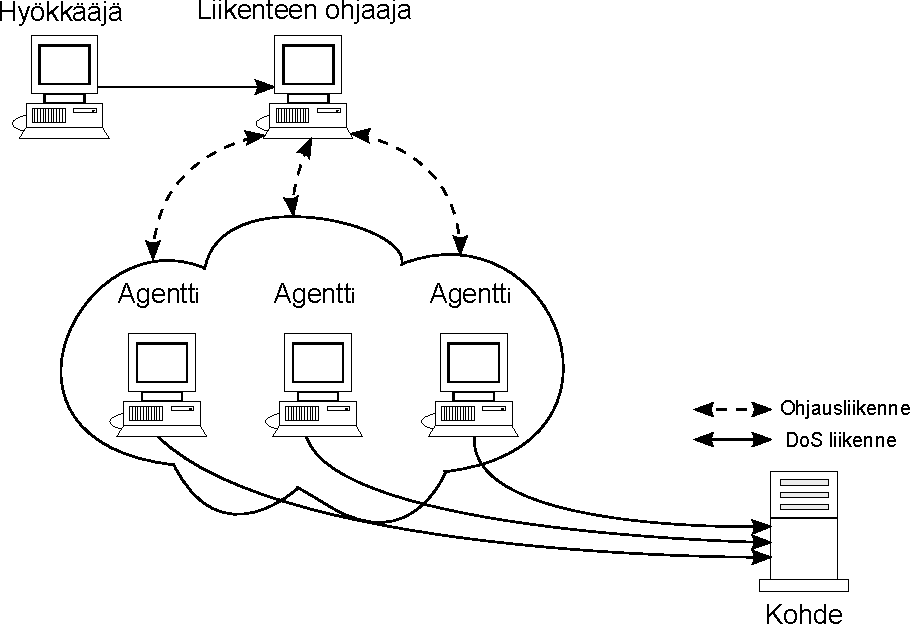
\includegraphics[width=12cm]{pics/perinteinen_ddos.pdf}
\caption{Perinteinen DDoS-verkosto}
\label{ddos1}
\end{figure}

Nykyisin enää harva DDoS-hyökkäyksessä käytetty verkko käyttää kuvan
\ref{ddos1} hierarkiaa sen heikon ohjattavuuden takia. Tämän tilalle
on tullut epäsuoraan käskyttämiseen perustuvat verkot, jotka käyttävät
viestien välittämiseen IRC-verkkoja (kuva \ref{ddos2}). IRC on
reaaliaikaiseen viestittämiseen tarkoitettu palvelu, jonka kautta
ihmiset pystyvät reaaliajassa kirjoittamaan ja lukemaan
viestejä. IRC-verkot koostuvat käyttäjistä ja IRC-kanavista, joille
käyttäjät voivat halutessana liittyä. Epäsuoran käskyttämisen
periaatteella toimivat verkot hyödyntävät näitä samoja
ominaisuuksia. Jokainen kone liittyy IRC-kanavalle, joka on yleensä
salasanalla suojattu. Kanavan kautta hyökkääjä voi antaa käskyjä
koneille. Tällä tavalla saadaan monia etuja verrattaessa suoraan
käskyttämiseen.  Ensinnäkin liikennettä ei pystytä enää tunnistamaan
poikkeavaksi, koska se on tavanomaista IRC-liikennettä. Toisekseen
käytettyä kanavaa voidaan vaihtaa lennosta, jolloin yhden kanavan
sulkeminen ei pysäytä verkon toimintaa. Näiden syiden takia
DDoS-hyökkäysten pysäyttäminen ennen niiden käynnistymistä on erittäin
vaikeaa \cite{DDOS}.

\begin{figure}[t]
\centering
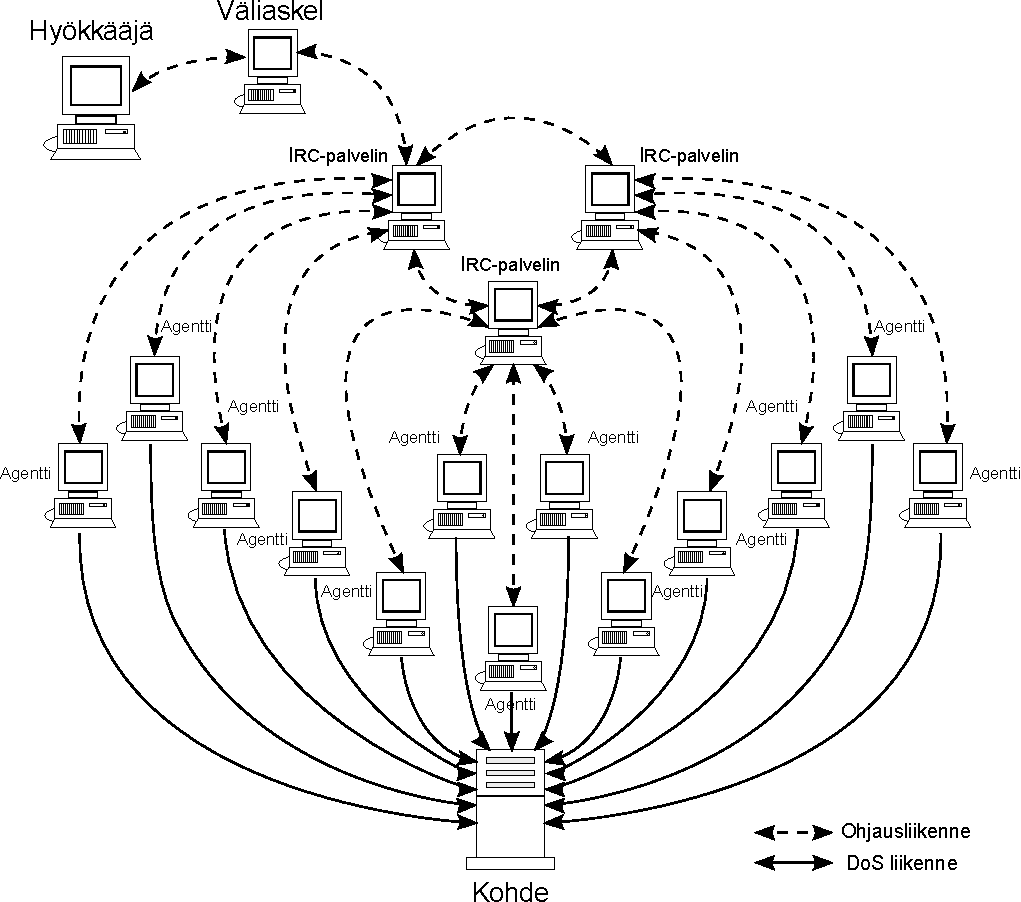
\includegraphics[width=12cm]{pics/ddos_uusi.pdf}
\caption{Nykyisin käytetty DDoS-verkosto}
\label{ddos2}
\end{figure}

\section{Remote-to-Local}

Remote-to-Local (lyh. \textit{R2L}) on hyökkäystyyppi, jossa hyökkääjä pyrkii
saamaan koneelle laajemmat oikeudet, kuin hänellä muuten
olisi. Tämä tapahtuu useimmiten käyttäen hyväksi järjestelmässä olevia
heikkouksia, joiden avulla hyökkääjä pääsee verkon yli murtautumaan
koneelle \cite{IDS}. Pahimmassa tapauksessa hyökkääjä saa hankittua koneelle
pääkäyttäjän oikeudet, jolloin koneen ja verkon resurssit ovat täysin
hyökkääjän käytettävissä.

Onnistuneet R2L-hyökkäykset ovat verkon ylläpitäjien kannalta pahimpia
mahdollisia, sillä niiden mahdollistamat tuhot ja aiheuttamat kustannukset ovat
huomattavasti suurempia verrattuna muihin hyökkäystyyppeihin \cite{IDSb}. Onnistunut R2L-hyökkäys saattaa
myös muut lähiverkon koneet vaaraan, sillä usein hyökkääjä pyrkii asentamaan
koneisiin ohjelmistoja, joiden avulla hyökkääjä pystyy ottamaan koneen haltuun
käyttäjän huomaamatta. Tällä tavoin osa aikaisemmin mainituista
zombverkostoista saa alkunsa.

Käytetyimmät Web-palvelinohjelmistot, Apache ja IIS, vastaavat noin 85~\%
kaikista käytetyistä palvelinsovelluksista. Näiden kahden lisäksi
BIND-\-ohjelmistoa käytetään valtaosassa nimipalvelimista. Ohjelmistojen yleisyydestä
johtuen yli puolet R2L-hyökkäyksen mahdollistavista heikkouksista onkin
löydetty näille alustoille \cite{IDS}. Useat haavoittuvaisuudet johtuvat
ohjelmointivirheistä, joiden johdosta hyökkääjä pystyy aiheuttamaan
sovellukseen muistin ylivuodon (engl. \textit{Buffer Overflow}). Tämä usein kaataa
sovelluksen tai saattaa sen sellaiseen tilaan, jossa hyökkääjä pystyy ajamaan
omia komentoja koneella. Kattava listaus löydetyistä haavoittuvuuksista ja näiden
korjauksista löytyy osoitteesta \url{www.cve.mitre.org/cve} \cite{CVE}.

Tunnetuilta R2L-hyökkäyksiltä suojautuminen on hyvin yksinkertaista, sillä
nykyinen trendi on, että haavoittuvuuden löytänyt taho ilmoittaa siitä
yleensä ensin
sovelluksen kehittäjille ennen julkista ilmoitusta. Siksi korjaus
haavoittuvuuteen on usein olemassa ennen kuin sitä on mahdollista hyödyntää \cite{IDSb}.
Vastuu jääkin verkon ylläpitäjälle, että käytetyt sovellukset ja 
suojausjärjestelmät pidetään ajan tasalla, sillä suurin osa onnistuneista hyökkäyksistä 
johtuu siitä, että tunnettuja tietoturva-aukkoja ei ole korjattu.

\section{User-to-Root}

User-to-Root (lyh. \textit{U2R}) hyökkäyksessä murtautuja pyrkii hankkimaan
koneelle pääkäyttäjän oikeudet. Tämä tapahtuu käyttäen järjestelmässä
olevia haavoittuvaisuuksia, joita ei ole paikattu. Useimmiten
hyökkäykset pohjautuvat koodausvirheisiin, jotka mahdollistavat
ylivuodon aiheuttamisen sekä odottamattomien syötteiden antamisen
\cite{IDS}. Käyttäjästä pääkäyttäjäksi hyökkäys eroaa R2L hyökkäyksestä
siten, että hyökkääjällä on jo valmiiksi pääsy koneelle tavallisen
käyttäjän oikeuksilla.

U2R-hyökkäykset ovat L2R-hyökkäysten ohella vaikeimpia torjua, jos kohteena
oleva järjestelmä on altis U2R-hyökkäyksille. Vaikea torjuttavuus johtuu siitä, että
usein hyökkäyksestä aiheutuva liikenne muistuttaa hyvin paljon normaalia
liikennettä, jonka vuoksi itsestään oppivat puolustusjärjestelmät eivät pysty
riittävän tarkasti erottamaan haitallista liikennettä normaalista \cite{U2R}.
Kehittyneimmilläkin järjestelmillä näiden hyökkäysten tunnistaminen on todella
heikkoa. Tämän on osoittanut useat eri tutkimushankkeet, jotka ovat käyttäneet
järjestelmiensä testaamiseen DARPAn simuloimaa verkkoliikennettä,
jossa olevat tietomurrot ja muu poikkeava toiminta on merkitty.
Parhaimmillaankin tunnistaminen on jäänyt 20 prosentin
paikkeille.

% TODO: Etsitäänpä tähän tietoa root exploiteista.
